\documentclass[dvipsnames,11pt]{article}
\usepackage{amsmath}

%Hey, if you're using this preamble it means that it was probably written by Stefano Graziosi (me). If you see something that doesn't make sense, feel free to email me at stefano.graziosi@studbocconi.it
%p.s. in case it's not already evident from the preamble, I'm not a professional LaTeX user, so I'm sure there are better ways to do things. I'm just trying to make it work.

%------------------------------------------------------------------------------
%           LAST UPDATE: 30-01-2025
%------------------------------------------------------------------------------

%I don't own copyright on anything, I just literally copied and pasted together a bunch of stuff.

%Credit goes to the original authors.

%------------------------------------------------------------------------------
%           Packages
%------------------------------------------------------------------------------

\usepackage{fancyhdr}
\usepackage[dvipsnames]{xcolor}
\usepackage[many]{tcolorbox}
\usepackage[all]{xy}
\usepackage{tcolorbox}
\usepackage{graphicx}
\usepackage{hyperref}
\usepackage{xcolor}    
\usepackage{wrapfig}
\usepackage{amsmath, amssymb, amsthm}
\usepackage{titlesec}
\usepackage{halloweenmath}
\usepackage{enumitem}
\usepackage{listings}
\usepackage{kantlipsum}
\usepackage{pdfpages}

\usepackage[T1]{fontenc}                            % Font Styling
\usepackage{lmodern,mathrsfs}


\usepackage{mathtools,amsthm,amssymb,amsfonts,bm}   % Math Presets
\usepackage{thmtools,amsmath}
\usepackage{array,tabularx,booktabs}                % Table Presets
\usepackage{graphicx,wrapfig,float,caption}         % Figure Presets
\usepackage{setspace,multicol}                      % Text Presets
\usepackage{tikz,physics}                           % Physics Presets

\usepackage{titlepic}
\usepackage{pdfpages}

%------------------------------------------------------------------------------
%           Geometry
%------------------------------------------------------------------------------

\usepackage[a4paper,margin=1in]{geometry}
%\usepackage[margin=1in]{geometry}

%------------------------------------------------------------------------------
%           Chapter and section formatting
%------------------------------------------------------------------------------

%\renewcommand{\chaptername}{Lecture}
%\renewcommand\thesection{P~\arabic{section}}

\renewcommand{\thefigure}{\thesection-\arabic{figure}}
\renewcommand{\thetable}{\thesection-\arabic{table}}

%------------------------------------------------------------------------------
%           Colours
%------------------------------------------------------------------------------

\definecolor{sgblue}{rgb}{0, 169, 211}
\definecolor{sggreen}{rgb}{0, 164, 0}
\definecolor{sgpurple}{rgb}{99, 0, 165}
\definecolor{sgyellow}{rgb}{255, 211, 0}
\definecolor{sgorange}{rgb}{255, 127, 20}

\definecolor{sbblue}{rgb}{219, 248, 254}
\definecolor{sbgreen}{rgb}{223, 255, 218}
\definecolor{sbpurple}{rgb}{241, 220, 255}

\definecolor{codegreen}{rgb}{0,0.6,0}
\definecolor{codegray}{rgb}{0.5,0.5,0.5}
\definecolor{codepurple}{rgb}{0.58,0,0.82}
\definecolor{backcolour}{rgb}{0.95,0.95,0.92}

%------------------------------------------------------------------------------
%           Environments
%------------------------------------------------------------------------------

%Standard \latex box

\newtcolorbox{mybox}[3][]
{
  colframe = #2!25,
  colback  = #2!10,
  coltitle = #2!20!black,  
  title    = {#3},
  #1,
}

%Standard "Problem" environment

\newtheorem{problem}{Problem}

%Personalised "Solution" environment

\newenvironment{solution}[1][\it{\textcolor{MidnightBlue}{Solution}}]{\textbf{#1. } }{\textcolor{MidnightBlue}{$\square$}}


% ----------------------------------------------------------------------
%           Special Environments 
% ----------------------------------------------------------------------

\newlength{\spacelength}
\settowidth{\spacelength}{\normalfont\ }
\declaretheoremstyle[
    headfont={\bfseries\sffamily\footnotesize},
    notefont={\normalfont},
    bodyfont={\normalfont},
    headpunct={\relax},%\newline,
    headformat={%
        \makebox[0pt][r]{\NAME\ \NUMBER\hspace{\marginparsep}}\hskip-\spacelength{\normalsize\NOTE}},
]{theorem}

\tcolorboxenvironment{theorem}{
  boxrule=0pt,
  boxsep=0pt,
  colback={White},
  enhanced jigsaw, 
  borderline west={1pt}{0pt}{ForestGreen},
  sharp corners,
  before skip=10pt,
  after skip=10pt,
  left=5pt,
  right=5pt,
  breakable,
}

\declaretheorem[style=theorem]{proposition}

\let\proof\relax
\let\endproof\relax

\declaretheoremstyle[
    headfont={\bfseries\sffamily\footnotesize},
    notefont={\normalfont},
    bodyfont={\normalfont},
    headpunct={\relax},%\newline,
    headformat={%
        \makebox[0pt][r]{\NAME\ \NUMBER\hspace{\marginparsep}}\hskip-\spacelength{\normalsize\NOTE}},
]{theorem}

\tcolorboxenvironment{proposition}{
  boxrule=0pt,
  boxsep=0pt,
  colback={White},
  enhanced jigsaw, 
  borderline west={1pt}{0pt}{Mulberry},
  sharp corners,
  before skip=10pt,
  after skip=10pt,
  left=5pt,
  right=5pt,
  breakable,
}

\declaretheorem[style=theorem]{theorem}

\let\proof\relax
\let\endproof\relax

\declaretheoremstyle[
    headfont={\small\scshape},
    notefont={\normalfont},
    bodyfont={\normalfont},
    headpunct={\relax},
    headformat={%
        \makebox[0pt][r]{\NAME\hspace{\marginparsep}}\hskip-\spacelength{\NOTE}},
]{proof}

\tcolorboxenvironment{proof}{
  boxrule=0pt,
  boxsep=0pt,
  blanker,
  borderline west={1pt}{0pt}{black},
  before skip=10pt,
  after skip=10pt,
  left=5pt,
  right=5pt,
  breakable,
}

\declaretheoremstyle[
    headfont={\footnotesize\itshape},
    notefont={\normalfont},
    bodyfont={\normalfont},
    headpunct={\relax},
    headformat={%
        \makebox[0pt][r]{\NAME\hspace{\marginparsep}}\hskip-\spacelength{\NOTE}},
]{claim}

\declaretheorem[
    style=proof,
    qed=\qedsymbol]{proof}

\declaretheorem[style=claim]{Intuition}

\theoremstyle{theorem}
\newtheorem{ques}{Question}

\theoremstyle{theorem}
\newtheorem{definition}{Definition}
\tcolorboxenvironment{definition}{
  boxrule=0pt,
  boxsep=0pt,
  colback={White},
  enhanced jigsaw, 
  borderline west={1pt}{0pt}{Cerulean},
  sharp corners,
  before skip=10pt,
  after skip=10pt,
  left=5pt,
  right=5pt,
  breakable,
}

\theoremstyle{theorem}
\newtheorem{lemma}{Lemma}
\tcolorboxenvironment{lemma}{
  boxrule=0pt,
  boxsep=0pt,
  blanker,
  borderline west={1pt}{0pt}{Rhodamine},
  before skip=10pt,
  after skip=10pt,
  sharp corners,
  left=5pt,
  right=5pt,
  breakable,
}

\theoremstyle{theorem}
\newtheorem{remark}{Remark}
\tcolorboxenvironment{remark}{
  boxrule=0pt,
  boxsep=0pt,
  colback={White},
  enhanced jigsaw, 
  borderline west={1pt}{0pt}{BurntOrange},
  before skip=10pt,
  after skip=10pt,
  sharp corners,
  left=5pt,
  right=5pt,
  breakable,
}

\theoremstyle{theorem}
\newtheorem{corollary}{Corollary}
\tcolorboxenvironment{corollary}{
  boxrule=0pt,
  boxsep=0pt,
%  colback={White!100!WildStrawberry},
  enhanced jigsaw,
  borderline west={1pt}{0pt}{WildStrawberry},
  before skip=10pt,
  after skip=10pt,
  sharp corners,
  left=5pt,
  right=5pt,
  breakable,
}

\theoremstyle{theorem}
\newtheorem{example}{Example}
\tcolorboxenvironment{example}{
  boxrule=0pt,
  boxsep=0pt,
  blanker,
  borderline west={1pt}{0pt}{Dandelion},
  before skip=10pt,
  after skip=10pt,
  sharp corners,
  left=5pt,
  right=5pt,
  breakable,
}


\theoremstyle{claim}
\newtheorem{intu}{Intuition}

\theoremstyle{claim}
\newtheorem{solu}{Solution}

%------------------------------------------------------------------------------
%           Code Listing Environment
%------------------------------------------------------------------------------

\lstdefinestyle{mystyle}{
    backgroundcolor=\color{backcolour},   
    commentstyle=\color{codegreen},
    keywordstyle=\color{magenta},
    numberstyle=\tiny\color{codegray},
    stringstyle=\color{codepurple},
    basicstyle=\ttfamily\footnotesize,
    breakatwhitespace=false,         
    breaklines=true,                 
    captionpos=b,                    
    keepspaces=true,                 
    numbers=left,                    
    numbersep=5pt,                  
    showspaces=false,                
    showstringspaces=false,
    showtabs=false,                  
    tabsize=2
}

\lstset{style=mystyle}

\setlength{\headheight}{25pt} % Non so perché ma senza questo da un piccolo errore

\pagestyle{fancy}
\fancyhf{} 
\fancyhead[L]{\textsc{\footnotesize{PhD in Economics and Finance} \\ \small{40313 Introd. to Probability}}} 
\fancyhead[R]{\textsc{\small Graziosi \\ Natalucci}} 
\fancyhead[C]{\textbf{Problem set 3}}
\fancyfoot[C]{\thepage} 
\renewcommand{\headrulewidth}{0.4pt} 
\renewcommand{\footrulewidth}{0pt}

\begin{document}

\section*{Question 1}

\textbf{1.} Let $X_1, X_2 , X_3$ be independent Gamma random variables with scale parameter $\lambda=2$ and shape parameters $k_1=1$, $k_2=2$ and $k_3=3$, respectively.

    \begin{enumerate}[label=\alph*.]
        \item Find the moment generating function of $X_i$ ($i=1,2,3$).
    
            \begin{solution}
    
                For $X\sim\Gamma(\lambda,k)$ the MGF is
                \[
                M_X(s)=E(e^{sX})=\left(\frac{\lambda}{\lambda-s}\right)^k,\qquad s<\lambda.
                \]
                Thus, with $\lambda=2$,
                \[
                M_{X_1}(s)=\frac{2}{2-s},\qquad
                M_{X_2}(s)=\left(\frac{2}{2-s}\right)^2,\qquad
                M_{X_3}(s)=\left(\frac{2}{2-s}\right)^3,\quad s<2.
                \]
                
            \end{solution}
            
        \item Find the probability distribution of $aX_i$ for $a>0$ ($i=1,2,3$).
    
            \begin{solution}
    
                Using $M_{aX}(s)=M_X(as)$,
                \[
                M_{aX_i}(s)=\left(\frac{2}{2-as}\right)^{k_i}
                =\left(\frac{2/a}{2/a-s}\right)^{k_i},
                \]
                which is the MGF of $\Gamma(2/a,k_i)$. Hence $aX_i\sim\Gamma(2/a,k_i)$.
                
            \end{solution}
            
        \item Find the probability distribution of $X_1+X_2+X_3$.
    
            \begin{solution}
    
                Independence and common $\lambda$ give
                \[
                M_{X_1+X_2+X_3}(s)=\prod_{i=1}^3 M_{X_i}(s)
                =\left(\frac{2}{2-s}\right)^{1+2+3}
                =\left(\frac{2}{2-s}\right)^{6}.
                \]
                Therefore $X_1+X_2+X_3\sim \Gamma(2,6)$.
                
            \end{solution}
            
        \item Find the probability distribution of $(X_1+X_2+X_3)/3$.
    
            \begin{solution}
    
                Let $S=X_1+X_2+X_3\sim\Gamma(2,6)$. For $a=1/3$,
                \[
                \frac{S}{3}\sim \Gamma\!\left(\frac{2}{1/3},\,6\right)=\Gamma(6,6).
                \]
                Equivalently, $M_{S/3}(s)=M_S(s/3)=\bigl(\tfrac{6}{6-s}\bigr)^6$.
                
            \end{solution}
            
        \item Find $E(X_1+X_2+X_3)^2$.
    
            \begin{solution}

                From $S\sim\Gamma(2,6)$,
                \[
                E(S)=\frac{6}{2}=3,\qquad V(S)=\frac{6}{2^2}=\frac{3}{2}.
                \]
                Thus
                \[
                E\bigl((X_1+X_2+X_3)^2\bigr)=E(S^2)=V(S)+[E(S)]^2
                =\frac{3}{2}+9=\frac{21}{2}=10.5.
                \]
                
            \end{solution}
            
    \end{enumerate}

%%%%%%%%%%%%%%%%%%%%%%%%%%%%%%%%%%%%%%%%%%%%

\section*{Question 2}

    \begin{enumerate}[label=\alph*.]
        \item Generate in Matlab or in Python a sample $(x_{1,i},x_{2,i},x_{3,i})$ with ($i=1,\dots,1000$), of size 1000 from the distribution of three independent Gamma random variables with scale parameter $\lambda=2$ and shape parameter $k=1$.

            \begin{solution}

\begin{lstlisting}[language=python]
import numpy as np

# Reproducibility
rng = np.random.default_rng(42)

# Sample of size 1000: three independent Gamma(k=1, scale=2)
n = 1000
scale = 2.0
X = rng.gamma(shape=1.0, scale=scale, size=(n, 3))
x1, x2, x3 = X.T
\end{lstlisting}
       
            \end{solution}

        \item Compute $y_i=x_{1,i}+x_{2,i}+x_{3,i}$.

            \begin{solution}
    
\begin{lstlisting}[language=python]
import matplotlib.pyplot as plt
from math import gamma as gamma_fn

y = x1 + x2 + x3  # In theory: y ~ Gamma(k=3, scale=2)

def gamma_pdf(x, k, theta):
    x = np.asarray(x)
    return np.where(
        x >= 0,
        (x ** (k - 1)) * np.exp(-x / theta) / (gamma_fn(k) * (theta ** k)),
        0.0,
    )

# Histogram for z with theoretical \Gamma(3,2) PDF
fig, ax = plt.subplots()
ax.hist(
    y,
    bins="fd",
    density=True,
    alpha=0.7,
    edgecolor="black",
    linewidth=0.6,
)

x_max = max(scale * 3 * 2.5, float(np.percentile(y, 99.5)))
grid = np.linspace(0.0, x_max, 600)
ax.plot(grid, gamma_pdf(grid, 3.0, scale), linewidth=2.0, label="Gamma(k=3, scale=2) PDF")

ax.set_title("Distribution of y = x1 + x2 + x3")
ax.set_xlabel("value")
ax.set_ylabel("density")
ax.grid(True, alpha=0.3, linestyle="--", linewidth=0.5)
for spine in ("top", "right"):
    ax.spines[spine].set_visible(False)
ax.legend(frameon=False)
fig.tight_layout()
plt.show()
\end{lstlisting}

                \begin{figure}[h]
                    \centering
                    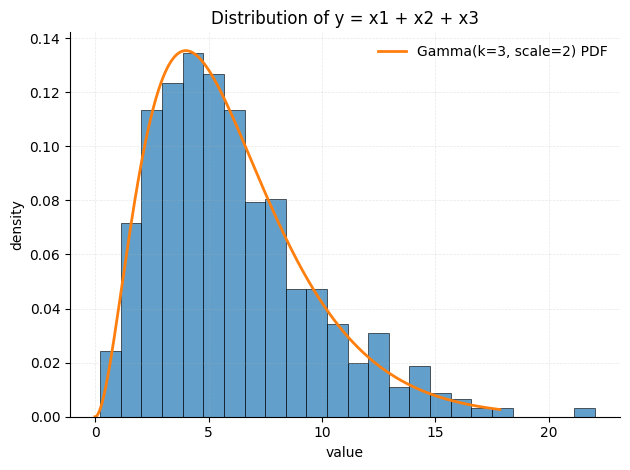
\includegraphics[width=0.5\linewidth]{q2b.png}
                    \caption{Distribution of \(y\)}
                    \label{fig:q2b}
                \end{figure}
                
            \end{solution}
            
        \item Generate a random sample $z_i$ ($i=1,\dots,1000$) from a Gamma distribution with scale parameter $\lambda=2$ and shape parameter $k=3$.

            \begin{solution}
    
\begin{lstlisting}[language=python]
import matplotlib.pyplot as plt
from math import gamma as gamma_fn

z = rng.gamma(shape=3.0, scale=scale, size=n)

def gamma_pdf(x, k, theta):
    x = np.asarray(x)
    return np.where(
        x >= 0,
        (x ** (k - 1)) * np.exp(-x / theta) / (gamma_fn(k) * (theta ** k)),
        0.0,
    )

# Histogram for z with theoretical \Gamma(3,2) PDF
fig, ax = plt.subplots()
ax.hist(
    z,
    bins="fd",
    density=True,
    alpha=0.7,
    edgecolor="black",
    linewidth=0.6,
)

x_max = max(scale * 3 * 2.5, float(np.percentile(z, 99.5)))
grid = np.linspace(0.0, x_max, 600)
ax.plot(grid, gamma_pdf(grid, 3.0, scale), linewidth=2.0, label="Gamma(k=3, scale=2) PDF")

ax.set_title("Distribution of z ~ Gamma(3, 2)")
ax.set_xlabel("value")
ax.set_ylabel("density")
ax.grid(True, alpha=0.3, linestyle="--", linewidth=0.5)
for spine in ("top", "right"):
    ax.spines[spine].set_visible(False)
ax.legend(frameon=False)
fig.tight_layout()
plt.show()
\end{lstlisting}

                \begin{figure}[ht]
                    \centering
                    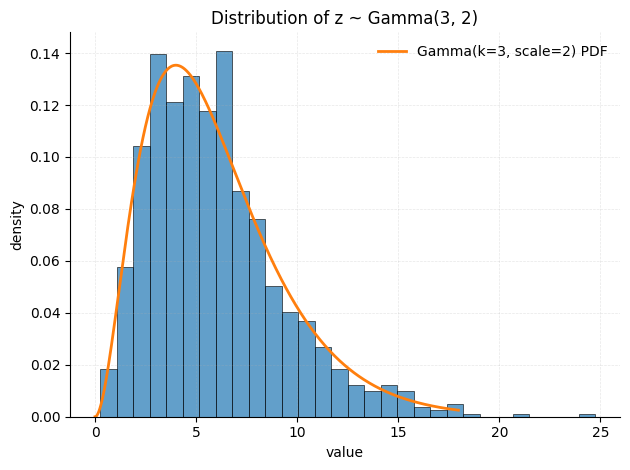
\includegraphics[width=0.5\linewidth]{q2c.png}
                    \caption{Distribution of \(z\)}
                    \label{fig:q2c}
                \end{figure}
                
            \end{solution}
            
        \item Compare the histogram of $y_1,\dots,y_{1000}$ with the histogram of $z_1,\dots,z_{1000}$.

            \begin{solution}
    
\begin{lstlisting}[language=python]
import matplotlib.pyplot as plt
from scipy import stats

combined = np.concatenate([y, z])
bins = np.histogram_bin_edges(combined, bins="fd")  # common bins for fair comparison

fig, ax = plt.subplots()
ax.hist(y, bins=bins, density=True, alpha=0.5, edgecolor="black", linewidth=0.6, label="y = x1 + x2 + x3")
ax.hist(z, bins=bins, density=True, histtype="step", linewidth=2.0, label="z ~ Gamma(3, 2)")

ax.set_title("Comparison: y vs z")
ax.set_xlabel("value")
ax.set_ylabel("density")
ax.grid(True, alpha=0.3, linestyle="--", linewidth=0.5)
for spine in ("top", "right"):
    ax.spines[spine].set_visible(False)
ax.legend(frameon=False)
fig.tight_layout()
plt.show()

# --- Distribution comparison tests ---
y_f = y[np.isfinite(y)]
z_f = z[np.isfinite(z)]

# 1) Kolmogorov-Smirnov two-sample test (global, bin-free)
ks = stats.ks_2samp(y_f, z_f, alternative="two-sided", method="auto")

# 2) Cramer-von Mises two-sample test (sensitive across the whole CDF)
cvm = stats.cramervonmises_2samp(y_f, z_f)

# 3) Wasserstein-1 distance (Earth Mover's Distance)
w1 = stats.wasserstein_distance(y_f, z_f)

print(f"KS test:                 D = {ks.statistic:.4f}, p = {ks.pvalue:.4g}")
print(f"Cramer-von Mises test:   T = {cvm.statistic:.4f}, p = {cvm.pvalue:.4g}")
print(f"Wasserstein-1 distance:  W-1 = {w1:.4f}")
\end{lstlisting}

                \begin{figure}[ht]
                    \centering
                    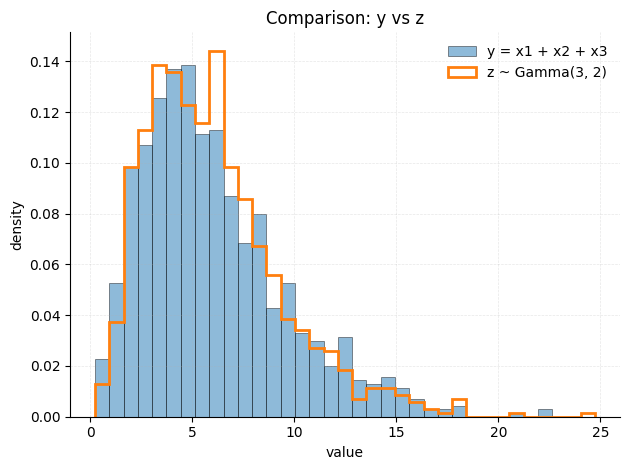
\includegraphics[width=0.5\linewidth]{q2d.png}
                    \caption{Comparison of \(y\) and \(z\)}
                    \label{fig:q2d}
                \end{figure}

                Across 1,000 draws, the two-sample tests show no evidence that the samples differ: KS $D=0.035$ ($p=0.573$) and Cramér–von Mises $T=0.106$ ($p=0.559$) both fail to reject the null that $y_i$ (sum of three $\Gamma(1,2)$) and $z_i$ (direct $\Gamma(3,2)$) come from the same distribution. The Wasserstein distance $W_1=0.204$ is small in natural units—about $0.204/\sqrt{12}\approx6\%$ of one standard deviation for $\Gamma(3,2)$—well within Monte Carlo variability for $n=1000$. 
                
                Overall, results are consistent with the additivity property of the Gamma family: $x_1+x_2+x_3 \sim \Gamma(3,2)$.
            
            \end{solution}
            
    \end{enumerate}

\end{document}
